\subsection{KNN}
Analisis de KNN
\\
Ahora vamos a analizar el algoritmo KNN (k vecinos mas cercanos) para distintos valores de k, fijando un valor de lamda, para ver como varia la efectividad (cantidad de aciertos) del algoritmo.
Vamos a probar el algormitmo KNN para los siguientes valores:

$\alpha$: 10  y k: 5, 50, 250.\\

Tambien, vamos a ejecutar para los valores anteriores, 5 pruebas iguales para cada uno, ya que el algoritmo varia la cantidad de aciertos segun que base de datos analice y no siempre da lo mismo.

Este algoritmo lo que hace es por cada imagen que queremos averiguar a que digito pertenece, vectorizarla, restarla a cada uno de los vectores imagen y calcular la norma2 para saber en cuanto difieren con cada una de las imagenes.
Todos esos resultados los vamos metiendo en una cola de prioridad que los ordena de menor a mayor, segun la diferencias entre la imagen que quiero averiguar a que digito pertenece y todas las imagenes de la base de datos.
\\
Luego lo que hacemos es agarrar los k primeros de la cola de prioridad y verificar a que digito se corresponden para luego saber cual es el digito que recibio mas 'votos' y ver si se produjo un acierto o no.
Por lo tanto, a mayor cantidad de vecinos (o sea, k) menor va a ser la cantidad de aciertos, ya que voy a empezar a mirar los elementos de menor prioridad de la cola, eso significa, que voy a empezar a contar las imagenes que mas difieren y eso me puede hacer que las chances de acertar el digito correcto disminuyan.
\\
El algoritmo KNN es muy efectivo ya que tiene aproximadamente entre 85\% y 90\% de aciertos. Pero su 'deficit' es que es muy lento a comparacion del algoritmo PCA. 







\subsubsection{Cantidad de vecinos}
Mover el k y presentar un analisis

\subsubsection{Mejoras en kNN}
Cortar el dataset en x valor y comparar para ver si mejora

\subsection{PCA}
Analisis de PCA
Ahora vamos a analizar el algoritmo del PCA.
Vamos a probar el algoritmo para distintas medidas de k y $\alpha$, que van a ser:\\
k: cantidad de vecinos a considerar en el algoritmo kNN.\\
$\alpha$: a la cantidad de componentes principales a tomar.

Vamos a probar el algoritmo para los siguientes valores:\\ \\
$\alpha$: 10  y k: 5, 20.\\
$\alpha$: 200 y k: 5, 20.\\
$\alpha$: 700 y k: 5, 20.\\
$\alpha$: 50  y k: 5, 25, 50, 100.\\


Lo que vamos a probar es fijando un valor de lamda, para que cantidad de vecinos vamos a tener la mayor cantidad de aciertos, y asi, maximizar la cantidad de aciertos.
Nosotros despues de aplicar el algoritmo pca, aplicamos el knn y armamos una cola de prioridad para los resultados de aplicar el algoritmo knn. Lo que se hace es agarrar dos imagenes, restarlas y aplicarle la norma2 para saber en cuanto difieren una imagen y la otra. El la cola de prioridad, estan adelante los valores mas chicos, o sea, las imagenes del test que mas cerca de coincidir estan con respecto a la imagen de la base de datos.
Por lo tanto, si elegimos mas cantidad de vecinos, lo que nos puede pasar son dos cosas:
1) Que sea beneficioso ya que a mayor cantidad de pruebas vamos a tener mas aciertos
2) Que sea malicioso ya que a mayor cantidad de pruebas vamos a obtener peores datos, o sea, vamos a mirar las imagenes que menos coiciden con la imagen de prueba de la base de datos.

La conclusion que llegamos es que a mayor cantidad de vecinos, el algoritmo empieza a funcionar peor, ya que estamos mirando los vecinos que menos coinciden con la base de datos, porque la cola de prioridad los ordena segun menos diferencias haya entre la foto obtenida y las fotos de la base de datos. 
Por lo tanto, cuanto mas vecinos exploro, menos cantidad de aciertos obtengo. Eso lo puedo ver a traves de las siguientes mediciones realizadas para distintos k vecinos y fijando un valor de lamda.

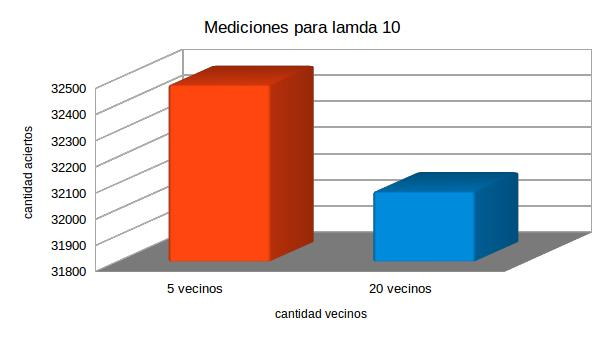
\includegraphics[scale=0.75]{lamda10.jpg}\\
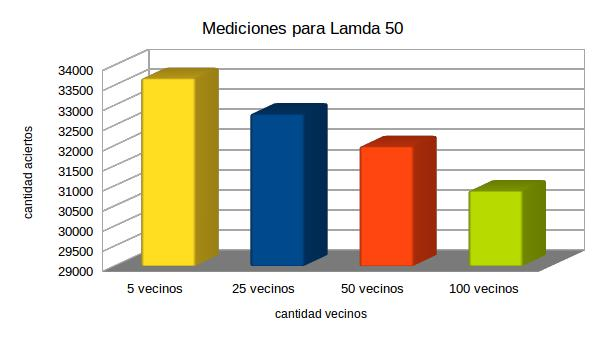
\includegraphics[scale=0.75]{lamda50.jpg}\\
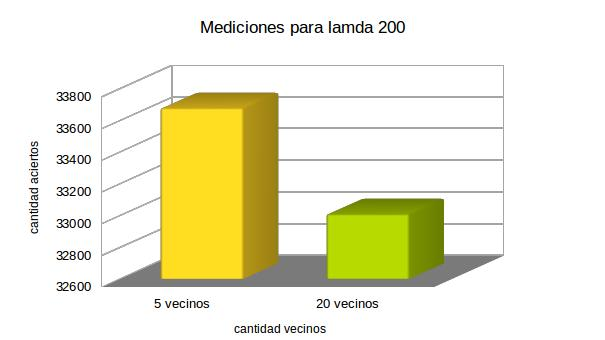
\includegraphics[scale=0.75]{lamda200.jpg}\\
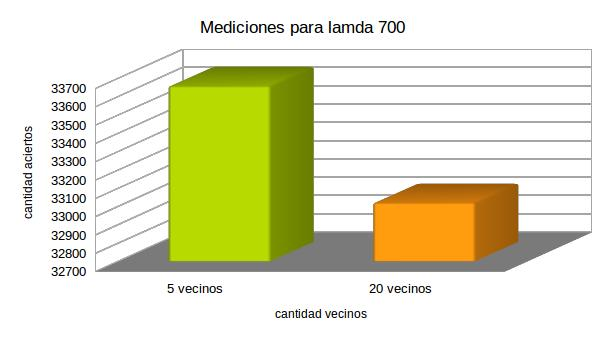
\includegraphics[scale=0.75]{lamda700.jpg}\\


Otra conclusion que sacamos es que para k=5 vecinos es la mejor cantidad de vecinos para obtener la mayor cantidad de aciertos. 
Ahora, ¿No seria mejor agarrar solo el primero de la cola de prioridad, o sea, k=1? 
Lo que podria pasar es que el unico vecino que agarremos, sea el mejor pero no alcance para saber cual es el digito de la imagen, ya que si no se acierta con el unico vecino que elegi, me podria fallar el digito del resultado y eso reduciria muchisimo la cantidad de aciertos.

\subsubsection{Lambda inicial}

\subsubsection{Algo mas que no me acuerde}
